\label{sec:r}
\subsection{Description}

The r-process occurs when neutron
densities and energies are high enough that the timescale for
neutron capture is much shorter than for $\beta^-$ decay.  Nuclear
evolution in this case does not follow the valley of stability but
instead passes on the neutron-rich side of the valley of stability.
Eventually as the neutron capture rate decreases the nuclei will have
an opportunity to \bminus\ decay back to the valley of stability.

Several pieces of relevant physics must be introduced.  One, nuclear
magic numbers, was already covered in Section~\ref{sec:nuc}.  The
lower neutron capture cross-sections of nuclei with magic numbers of
neutrons has a significant impact on the flow of nuclei toward
increasing $A$ in the r process.  Another important piece 
 is the so-called
``neutron drip line.''  A nucleus with a given $Z$ has a maximum
number of neutrons it can keep bound to it; any additional neutrons
that are captured once this number is reached causes a neutron to be
emitted (or ``dripped'') from the nucleus.  So neutron capture at 
the neutron drip line permits no change in $A$ or $Z$.  
This maximum number of neutrons a nucleus can hold expressed as a
function of $Z$ describes the neutron drip line and it is the hard
edge seen on the neutron-rich side of the CON.  Also relevant is
photodisintegration.  At the temperatures expected for the r-process
photons have enough energy to liberate neutrons from the nucleus:
$^A_Z$X$+\gamma \rightarrow _{\ \ \ Z}^{A-1}$X$+n$.  This process
works against neutron capture.

A qualitative description of the r-process follows.  Because the 
r-process does not follow the valley of stability like the
s-process does, it is more difficult to describe a canonical r-process
trajectory than for the s-process.  Instead a general picture
will be described illustrating the general principles that determine
each of a multitude of r-process trajectories.  A
rapid succession of neutron captures on seed nuclei causes a
signficant neutron enrichment of the nuclei.  As this proceeds there
are several things that can happen.  Additional neutron captures can
further increase the $A$ of the nuclei.  A \bminus\ decay even can
happen. Photodisintegration can
remove neutrons from the nucleus.  Nuclei can run up against the
neutron drip line, where they remain until a \bminus\ decay or
photodisintegration event move them off the drip line.  Nuclei can
get a magic number of neutrons, where lower neutron capture
cross-sections keep them from progressing as quickly to the next $A$.
These highlight some of the important individual events that can
happen in the r-process. After the neutron source is turned off the 
neutron-rich nuclei are
able to \bminus\ decay to the valley of stability.  
%Because of this
%beeline to the valley of stability after a neutron source is turned
%off, there is only one r-process nuclide 


A simple r-process model for $T\geq 1$ GK and constant $N_n \geq 10^{21}$
cm$^{-3}$ is given in \cite{iliadis2008}.  For temperatures and
neutron densities this high, both neutron capture and
photodisintegration occure much faster than \bminus\ decays.  In this
case the abundance evolution of a species $^A_Z$X is given by
\begin{multline}
\frac{N(Z,A+1)}{N(Z,A)} = - N_nN(Z,A) \langle \sigma v \rangle_{Z,A} \\
+N(Z,A+1)\times\lambda_\gamma (Z,A+1)
\end{multline}
where $N(Z,A)$ is the number density of  nuclide $^A_Z$X, $\langle 
\sigma v \rangle_{Z,A}$ is the neutron
capture reaction rate per particle pair for the same nuclide, and
$\lambda_\gamma (Z,A+1)$ is the photodisintegration constant for
nuclide  $^{A+1}_{\ \ \ Z}$X. 
In the case that the forward and reverse
reactions of neutron capture and photodisintegration reach equilibrium
the abundance ratios for two adjacent isotopes can be expressed by the
Saha equation
\begin{multline}
\label{eq:saha}
\frac{N(Z,A+1)}{N(Z,A)} =N_n\left(\frac{h^2}{2\pi
(Am_{n})kT}\right)^{3/2} \times \\
\frac{2j_{Z,A+1}+1}{(2j_{Z,A}+1)(2j_{n}+1)}
\frac{G^{\textrm{norm}}_{Z,A+1}}{G^{\textrm{norm}}_{Z,A}}e^{Q_{n\gamma}/kT}
\end{multline}
where $j_{Z,A} (j_n)$ is the angular momentum quantum number for
$^{A}_{Z}$X ($n$, a single neutron), $G^{\textrm{norm}}_{Z,A}$ is a normalized parition
function (in what follows both $j_{Z,A}$ and
$G^{\textrm{norm}}_{Z,A}$ are largely ignored and so no more specific
definitions are given), and $Q_{n\gamma}$ is the Q-value for the forward 
neutron capture
reaction on $^{A}_{Z}$X (equivalently the neutron separation energy of
$^{A+1}_{\ \ \ Z}$X). Equation~\ref{eq:saha} can be used 
for a specific $T$ and $N_n$ to find what value of 
$Q_{n\gamma}$  gives $N(Z,A+1) \approx N(Z,A)$.
For example, \cite{iliadis2008} calculates that with $T=1.25$ GK and 
$N_n=10^{22}$ cm$^{-3}$ and neglecting spin and partition function terms
$N(Z,A+1) \approx N(Z,A)$ for $Q_{n\gamma}\approx$ 3 MeV.  Generally,
$Q_{n\gamma}$ is larger closer to the valley of the stability and
smaller closer to the neutron drip line (\citealt{iliadis2008}) and
so, for a given isotopic chain, if $Q_{n\gamma}$ is 3 MeV somewhere
between the valley of stability and the neutron drip line then closer
to the valley of stability $Q_{n\gamma}> 3$  MeV and $N(Z,A+1) >
N(Z,A)$; similarly, closer to the neutron drip line $Q_{n\gamma}< 3$
MeV and $N(Z,A+1) < N(Z,A)$.  Thus in this simple picture (no spin or
partition function considerations and the assumption  that neutron capture and
photodisintegration proceed faster than \bminus\ decays)
the r-process  tries to pull abundances in a
given isotopic chain toward a specific $^A_Z$X which has a
$Q_{n\gamma}$ value close to that which permits $N(Z,A+1) \approx N(Z,A)$. 

%An important extension to this model to make it more physically
%palatable is that, for isotopes adjacent in $A$, isotopes with even
%numbers of neutrons have smaller $Q_{n\gamma}$ values than those with
%odd numbers of neutrons.  

\bminus\ decays move nuclides from one isotopic chain to the next
higher one in $Z$.  Looking at elements as a whole \cite{iliadis2008}
has a simple model showing the movement of nuclides from one element
to the next.  Defining $N_Z$ to be the abundance of a given {\it
element} (not nuclide)
\begin{equation}
\label{eq:lambdaz}
\frac{dN_Z}{dt} = - \lambda_ZN_Z + \lambda_{Z-1}N_{Z-1}
\end{equation}
where
\begin{equation}
\label{eq:th}
\lambda_Z = \sum_Ap(Z,A)\lambda_\beta (Z,A)
\end{equation}
and $p(Z,A) = N(Z,A)/N_Z$ is the normalized abundance distribution for a given
isotopic chain for a given $T$ and $N_n$ and $\lambda_\beta (Z,A)$ is
the \bminus\ decay constant for a given species.
Equation~\ref{eq:lambdaz} has two terms, the first of which describes
isotopes of element $Z$ decaying off the isotopic chain and the second
of which describes isotopes of element $Z-1$ decaying onto the
isotopic chain $Z$.  Equations~\ref{eq:lambdaz} and {eq:th} taken
together with boundary conditions $N_Z(t=0)=N_0$ for some $Z=Z_0$  and
$N_Z(t=0)=0$ for $Z\neq Z_0$.  The solution, as given in
{\cite{iliadis2008} is
\begin{equation}
N_{Z_0}(t) = N_0 e^{-\lambda_{Z_0} t}
\end{equation}
\begin{multline}
\label{eq:pi}
N_Z(t) = N_0 \sum_{i=Z_0}^Z e^{-\lambda_i
  t}\frac{\lambda_i}{\lambda_Z} \\
\times \prod_{\substack{j=Z_0\\ j\neq i}} \frac{\lambda_j}{\lambda_j -
  \lambda_i}~~~~\textrm{for}~Z\neq Z_0
\end{multline}
provided all values of $\lambda_j$ are different.  
We can see from Equation~\ref{eq:pi} that $N_Z$ and $\lambda_Z$ are
inversely related; so the higher the decay rate the lower the
abundance and vice-versa, which makes sense.  More important to note
is that the equations are self-regulating in that they work towards
achieving a constant flow from one isotopic chain to the next via
\bminus\ decays (\citealt{iliadis2008}); if indeed such a constant
flow is established then we get
\begin{equation}
\lambda_ZN_Z \approx ~ \textrm{const}.
\end{equation}
Thus there can be pile ups of elements with low $\lambda_Z$.

I can add more about magic numbers if I want.  But talk about with the
peaks in abundances below

As was mentioned in Section~\ref{sec:s} there are some stable nuclides
that are inaccessible by the s-process due to ``weak links'' in the
reaction chains that would otherwise contribute to their formation,
the weak links being nuclides with fast decay rates that \bminus\
decay back to the valley of stability; the formation of these nuclides
is completely attributable to the r-process.  Similarly, there are
some nuclides that are inaccessible by the r-process and whose
formation can be completely attributed to the s-process.  {\bf Figure}
shows such a nuclide.  r-process reation chains would end up at ?? and
thus would be unable to access any isobars of ?? with higher $Z$.  ??
is shielded from the r-process by ?? and thus cannot be formed by the
s-process.



 There are several compelling evidences that something like the
 r-process as described here occurs in nature.  The existence of
 nuclides inaccessible by the s-process is one, as discussed above.  
Another evidence  can be seen in
the abundance peaks in {\bf Figure r-process peak offset}.  As
mentioned in Section~\ref{sec:s} 
the lower neutron capture cross-section of nuclides with a magic
number of neutrons there is a pile up of the abundances of these
nuclides.   A similar thing happens in the r-process.  Lower neutron
 capture cross sections as well as smaller \bminus\ decay rates
 relative to their CON neighbors
 (because the neutrons are in a stable configuration) causes a pile up
 along the neutron magic number isotones. Because the r-process isn't limited to
 following the valley of stability as neutrons are added to nuclei
 there are pile ups of several nuclides for each magic number.  After
 neutron captures have stopped these nuclei will \bminus\ decay back
 to the valley of stability, increasing in $Z$ while decreasing in $N$
 to maintain $A$.  Because the r-process can access nuclei with magic
 numbers of neutrons with small $A$ than the s-process, the resulting
 peaks in r-process abundances will be at smaller $A$ than the
 s-process abundances. Figure~\ref{fig:peaks} shows this difference
 between the s-process and r-process peaks.  The s-process peaks
 (primarily shown with red circles)  occur at
 higher $A$ than the r-process peaks (primarily shown with green
 diamonds).  
Additionally, because the number of neutron magic
number nuclei accessible to the r-process is greater than the
corresponding nuclei for the s-process, the r-process peaks are wider
than the s-process peaks, which is also seen in
 Fgiure~\ref{fig:peaks}.  
The existence of these peaks is one of the
strongest evidences for the existence of something like the r-process.
\begin{figure*}
\centering
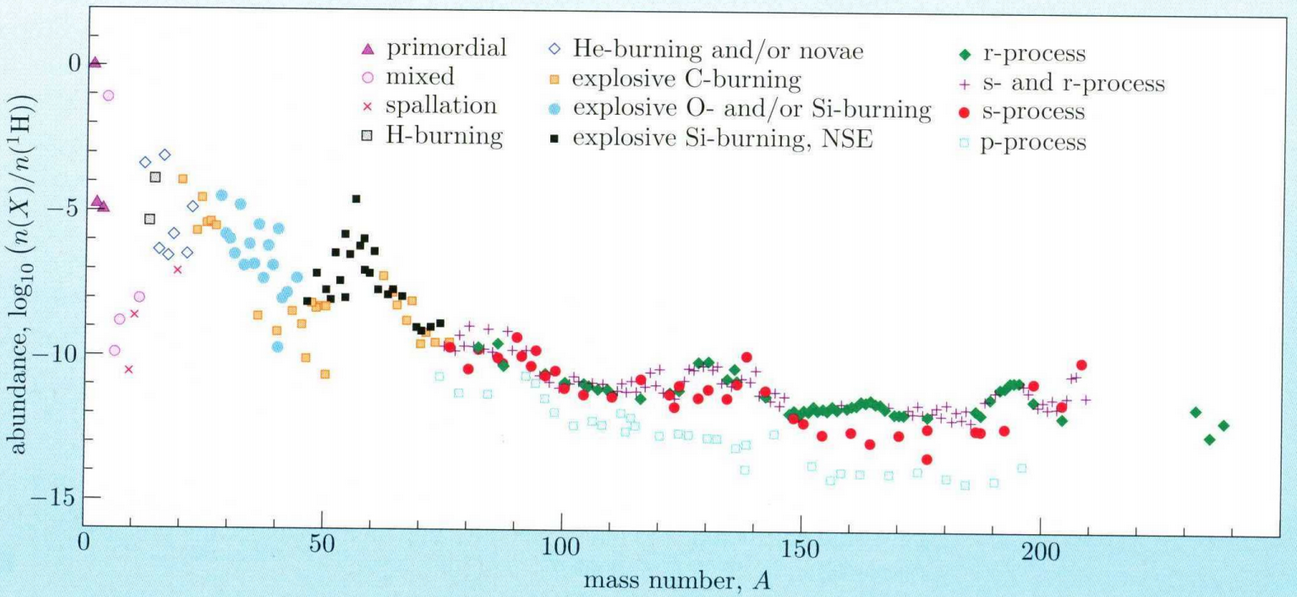
\includegraphics[width=6in]{pdf/peaks.png}
\caption{\label{fig:peaks} Measured abundances of stable nuclides
 along with their likely source.  Many different sources are shown but
 most relevant to our discussion are those nuclides above the iron
 peak
 ($A\gtrsim75$),
 where the s- and r-process (and p-process to a lesser degree) are the
 synthesis sources.  Green diamonds are those nuclides which are
 primarily produced by the r-process, red circles those primarily
 produced by the s-process, and purple crosses those produced by a
 mixture of the two processes.  From~\cite{ryan2010}.}
\end{figure*}

Another strong evidence for something like the r-process being in
operation in the universe is the natural existence of Th and Ur.
These elements cannot be created by the s-process because of the
s-process termination described by Equations~\ref{eq:firsttermination}
and~\ref{eq:secondtermination}; their creation requires a process that
can bridge over nuclides with short decay times.





%Waiting time approximation (also called primary r-process: \citealt{meyer1994}).

Dynamic r-process calculation (Nn, T descreatese with time)


\subsection{Proposed Sites}

Entropy discussion of Meyer?

There are two main roposed r-processing sites which are core-collapse
supernovae and neutron star mergers.  Both involve transient, cataclysmic events
with high neutron densities and high temperatures, important
conditions for having neutron captures rates higher than \bminus\
decay rates.  Before a detailed explanation of each proposed site is
given I will first examine some observational constraints on r-process
sites. One is observations of old stars with very low
metallicity ([Fe/H]$\lesssim-2.5$).  These stars consistently show
abundances consistent with production from the r-process with little
to no contribution from the s-process (\citealt{truranetal2002}.  
Figure~\ref{fig:old} shows 
total heavy element abudances of a metal poor  Galactic halo star with
the solar system r-process abundances scaled to fit.  The plot itself as well
as the residual plot show that the r-process solar system abundances
fit remarkably well for elements past Ba ($A\approx 135$).  \cite{truranetal2002} say
that such a match between solar system r-process abundances and halo
star heavy metal abundances is seen for most stars with
[Fe/H]$\lesssim-2.5$.  These data provide very strong evidence that
the r-process was active in the early galaxy and gives us clues as to
where r-processing happens.  Since these stars were enriched in
r-process elements during their formation and they formed at such
early times in the Galactic history it can be concluded that something
related to the 
massive stars present in the early galaxy, which live only a short
time, is the site for the r-process.  Also the mismatch between low
metallicity halo star abundances and solar system r-process abundances
below $A\approx135$ suggests some variety in the r-process: either
different sites or different conditions at the same site. 
%The fact
%that $^{138}$Ba has a magic number (82) of neutrons may be a reason
%why different sites or conditions have a turnover here.  As
%mentioned before in r-processing there is a pile up of nuclides around
%nuclides with neutron magic numbers.  This is in part due to the
%difficulty nuclides have in capturing an additional neutron to pass
%the neutron magic number to higher $N$ nuclei.  Because of this,
%nuclei often undergo several successive \bminus\ decays and neutron
%captures before moving past the neutron magic number.  
\begin{figure}
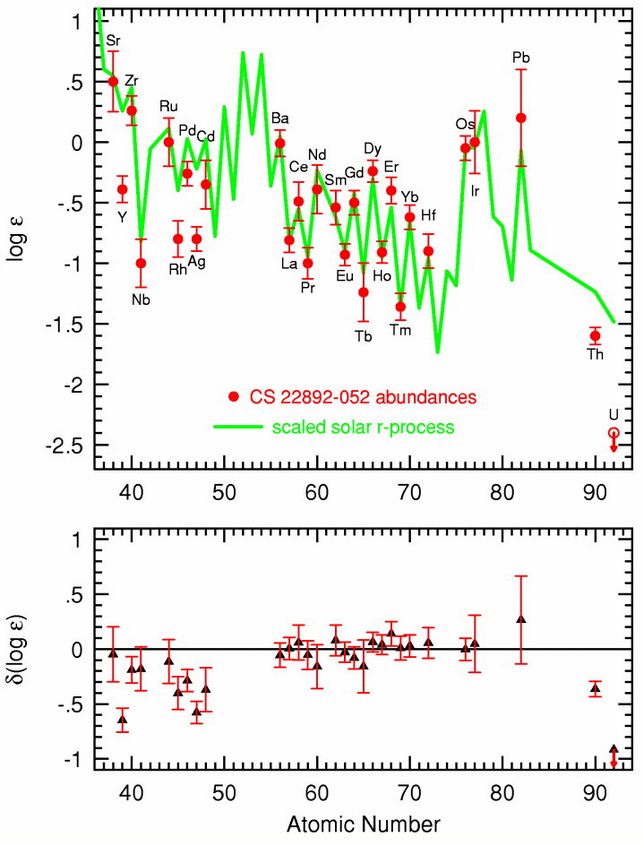
\includegraphics[width=\linewidth]{pdf/oldstar.png}
\caption{\label{fig:old} Data points represent measured heavy element
abundances from the metal-poor Galactic halo star CS 22892-052 while
the solid line represents the solar system r-abundance measurements,
scaled to fit the data points.  $\log \epsilon (x) \equiv log(N_x/N_H) +
12.0$ for a given element $x$.  Residuals are shown in the lower
plot.  From~\cite{truranetal2002}.}
\end{figure}

Let us examine the requirements of the r-process.  Neutron captures
must proceed at a rate quicker than \bminus\ decay rates but also must
only happen for a limited amount of time, otherwise it is easy to
image scenarios where nuclides are ``over-processed'' and become very
heavy on average with a large abundance near Pb end of the valley of
stability and fission products of heavier nuclei, which is not seen.
